\documentclass{beamer}

\pdfmapfile{+sansmathaccent.map}


\mode<presentation>
{
  \usetheme{Warsaw} % or try Darmstadt, Madrid, Warsaw, Rochester, CambridgeUS, ...
  \usecolortheme{crane} % or try seahorse, beaver, crane, wolverine, ...
  \usefonttheme{serif}  % or try serif, structurebold, ...
  \setbeamertemplate{navigation symbols}{}
  \setbeamertemplate{caption}[numbered]
} 


%%%%%%%%%%%%%%%%%%%%%%%%%%%%
% itemize settings

\definecolor{myhotpink}{RGB}{255, 80, 200}
\definecolor{mywarmpink}{RGB}{255, 60, 160}
\definecolor{mylightpink}{RGB}{255, 80, 200}
\definecolor{mypink}{RGB}{255, 30, 80}
\definecolor{mydarkpink}{RGB}{155, 25, 60}
\definecolor{myblue}{RGB}{240, 240, 255}
\definecolor{mydarkblue}{RGB}{60, 160, 255}
\definecolor{mygreen}{RGB}{0, 200, 0}
\definecolor{mygreen2}{RGB}{245, 255, 230}
\definecolor{mygray}{gray}{0.8}


\definecolor{mydarkcolor}{RGB}{60, 25, 155}
\definecolor{mylightcolor}{RGB}{130, 180, 250}

\setbeamertemplate{itemize items}[default]

\setbeamertemplate{itemize item}{\color{mywarmpink}$\blacksquare$}
\setbeamertemplate{itemize subitem}{\color{mydarkblue}$\blacktriangleright$}
\setbeamertemplate{itemize subsubitem}{\color{mygray}$\blacksquare$}



\setbeamercolor{palette quaternary}{fg=white,bg=mydarkcolor}
\setbeamercolor{titlelike}{parent=palette quaternary}

\setbeamercolor{palette quaternary2}{fg=black,bg=mylightcolor}
\setbeamercolor{frametitle}{parent=palette quaternary2}



\setbeamerfont{frametitle}{size=\Large,series=\scshape}
\setbeamerfont{framesubtitle}{size=\normalsize,series=\upshape}


%%%%%%%%%%%%%%%%%%%%%%%%%%%%
% block settings

\setbeamercolor{block title}{bg=red!50,fg=black}

\setbeamercolor*{block title example}{bg=mygreen!40!white,fg=black}

\setbeamercolor*{block body example}{fg= black,
bg= mygreen2}


%%%%%%%%%%%%%%%%%%%%%%%%%%%%
% URL settings
\hypersetup{
    colorlinks=false,
    linkcolor=blue,
    filecolor=blue,      
    urlcolor=blue,
}

%%%%%%%%%%%%%%%%%%%%%%%%%%

\renewcommand{\familydefault}{\rmdefault}

\usepackage{amsmath}
\usepackage{mathtools}

\usepackage{subcaption}


\newcommand{\mydate}{Spring 2022}
\newcommand{\mygit}{\textcolor{blue}{\href{https://github.com/SergeiSa/Computational-Intelligence-Slides-Spring-2022}{github.com/SergeiSa/Computational-Intelligence-Slides-Spring-2022}}}

\newcommand{\bo}[1] {\mathbf{#1}}
\newcommand{\R} {\mathbb{R}}
\DeclareMathOperator*{\argmin}{arg\,min}


%%%%%%%%%%%%%%%%%%%%%%%%%%%%
% code settings

\usepackage{listings}
\usepackage{color}
% \definecolor{mygreen}{rgb}{0,0.6,0}
% \definecolor{mygray}{rgb}{0.5,0.5,0.5}
\definecolor{mymauve}{rgb}{0.58,0,0.82}
\lstset{ 
  backgroundcolor=\color{white},   % choose the background color; you must add \usepackage{color} or \usepackage{xcolor}; should come as last argument
  basicstyle=\footnotesize,        % the size of the fonts that are used for the code
  breakatwhitespace=false,         % sets if automatic breaks should only happen at whitespace
  breaklines=true,                 % sets automatic line breaking
  captionpos=b,                    % sets the caption-position to bottom
  commentstyle=\color{mygreen},    % comment style
  deletekeywords={...},            % if you want to delete keywords from the given language
  escapeinside={\%*}{*)},          % if you want to add LaTeX within your code
  extendedchars=true,              % lets you use non-ASCII characters; for 8-bits encodings only, does not work with UTF-8
  firstnumber=0000,                % start line enumeration with line 0000
  frame=single,	                   % adds a frame around the code
  keepspaces=true,                 % keeps spaces in text, useful for keeping indentation of code (possibly needs columns=flexible)
  keywordstyle=\color{blue},       % keyword style
  language=Octave,                 % the language of the code
  morekeywords={*,...},            % if you want to add more keywords to the set
  numbers=left,                    % where to put the line-numbers; possible values are (none, left, right)
  numbersep=5pt,                   % how far the line-numbers are from the code
  numberstyle=\tiny\color{mygray}, % the style that is used for the line-numbers
  rulecolor=\color{black},         % if not set, the frame-color may be changed on line-breaks within not-black text (e.g. comments (green here))
  showspaces=false,                % show spaces everywhere adding particular underscores; it overrides 'showstringspaces'
  showstringspaces=false,          % underline spaces within strings only
  showtabs=false,                  % show tabs within strings adding particular underscores
  stepnumber=2,                    % the step between two line-numbers. If it's 1, each line will be numbered
  stringstyle=\color{mymauve},     % string literal style
  tabsize=2,	                   % sets default tabsize to 2 spaces
  title=\lstname                   % show the filename of files included with \lstinputlisting; also try caption instead of title
}

%%%%%%%%%%%%%%%%%%%%%%%%%%%%
% tikz settings

\usepackage{tikz}
\tikzset{every picture/.style={line width=0.75pt}}

%%%%%%%%%%%%%%%%%%%%%%%%%%%%

\usepackage{qrcode}



\title{Linear inequality representation of convex domains}
\subtitle{Computational Intelligence, Lecture 7}
\author{by Sergei Savin}
\centering
\date{\mydate}

\begin{document}
\maketitle


\begin{frame}{Content}

\begin{itemize}
\item Convex polytopes
\item Half-spaces
\begin{itemize}
\item Definition
\item Construction. Simple case
\item Construction. General case
\item Combination
\item H-representation
\item V-representation
\end{itemize}
\item Linear approximation of convex regions
\item Homework
\end{itemize}

\end{frame}



\begin{frame}{Convex polytopes}
% \framesubtitle{Parameter estimation}
\begin{flushleft}

Before defining what a convex polytope is, let us look at examples:


\begin{figure}
\centering
\begin{minipage}{.25\textwidth}
  \centering
  
\begin{tikzpicture}[thick,scale=3]
    \coordinate (A1) at (0,0);
    \coordinate (A2) at (0.6,0.2);
    \coordinate (A3) at (1,0);
    \coordinate (A4) at (0.4,-0.2);
    \coordinate (B1) at (0.5,0.5);
    \coordinate (B2) at (0.5,-0.5);
    %
    \begin{scope}[thick,dashed,,opacity=0.6]
        \draw (A1) -- (A2) -- (A3);
        \draw (B1) -- (A2) -- (B2);
    \end{scope}
    %
    \draw[fill=myhotpink,   opacity=0.6] (A1) -- (A4) -- (B1);
    \draw[fill=mydarkgray, opacity=0.6] (A1) -- (A4) -- (B2);
    \draw[fill=mylightpink,     opacity=0.6] (A3) -- (A4) -- (B1);
    \draw[fill=mydarkpink,      opacity=0.6] (A3) -- (A4) -- (B2);
    \draw (B1) -- (A1) -- (B2) -- (A3) --cycle;
\end{tikzpicture}

%   \captionof{figure}{Convex domain}
\end{minipage}%
\begin{minipage}{.45\textwidth}
  \centering

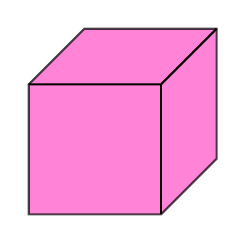
\begin{tikzpicture}[x=0.55pt,y=0.55pt,yscale=-1,xscale=1]
%uncomment if require: \path (0,300); %set diagram left start at 0, and has height of 300
%Shape: Cube [id:dp8775233577412218] 
\draw [fill=myhotpink,   opacity=0.7] (71.5,108.6) -- (108.1,72) -- (195,72) -- (195,157.4) -- (158.4,194) -- (71.5,194) -- cycle ; \draw   (195,72) -- (158.4,108.6) -- (71.5,108.6) ; \draw   (158.4,108.6) -- (158.4,194) ;
\end{tikzpicture}

%   \captionof{figure}{Non-convex domain}
\end{minipage}
\begin{minipage}{.35\textwidth}
  \centering

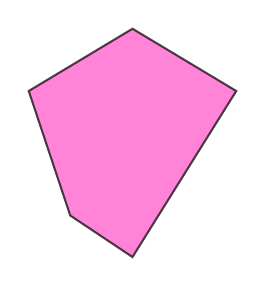
\begin{tikzpicture}[x=0.75pt,y=0.75pt,yscale=-1,xscale=1]
%uncomment if require: \path (0,300); %set diagram left start at 0, and has height of 300
%Shape: Polygon [id:ds951364720833231] 
\draw [fill=myhotpink,   opacity=0.7] (340,71) -- (390,101) -- (340,181) -- (310,161) -- (290,101) -- cycle ;
\end{tikzpicture}

%   \captionof{figure}{Non-convex domain}
\end{minipage}
\begin{minipage}{.25\textwidth}
  \centering

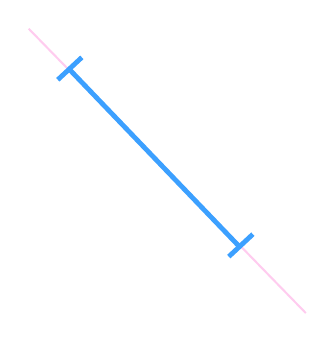
\begin{tikzpicture}[x=0.75pt,y=0.75pt,yscale=-1,xscale=1]
%uncomment if require: \path (0,300); %set diagram left start at 0, and has height of 300
%Straight Lines [id:da23716511791848993] 
\draw [color=myhotpink  ,draw opacity=0.29 ]   (135,67) -- (268.5,204) ;
%Straight Lines [id:da07398036110019657] 
\draw [color=mydarkblue  ,draw opacity=1, line width=1.75pt ]   (155,87) -- (237,172.5) ;
%Straight Lines [id:da4002272137050389] 
\draw [color=mydarkblue  ,draw opacity=1, line width=1.75pt ]   (149,91.6) -- (160.6,80.8) ;
%Straight Lines [id:da5388486506254657] 
\draw [color=mydarkblue  ,draw opacity=1, line width=1.75pt ]   (231.4,176.8) -- (243,166) ;
\end{tikzpicture}

%   \captionof{figure}{Non-convex domain}
\end{minipage}
\end{figure}
 
\end{flushleft}
\end{frame}


\begin{frame}{Convex polytopes}
% \framesubtitle{Parameter estimation}
\begin{flushleft}

You can think of polytopes as geometric figures (or continuous sets of points) with linear edges, faces and higher-dimensional analogues.

\bigskip

\begin{definition}
 Convex polytopes are polytopes whose every two points can be connected with a line that would lie in the polytope. They can be bounded or unbounded.
\end{definition}
 
\end{flushleft}
\end{frame}


\begin{frame}{Half-spaces}
\framesubtitle{Definition}
\begin{flushleft}

We can define half-space as a set of all points $\mathbf{x}$, such that $\mathbf{a}^\top \mathbf{x} \leq b$. It has a very clear geometric interpretation. In the following image, the filled space is \textbf{not} in the half space.

\begin{figure} [h!]
\begin{center}

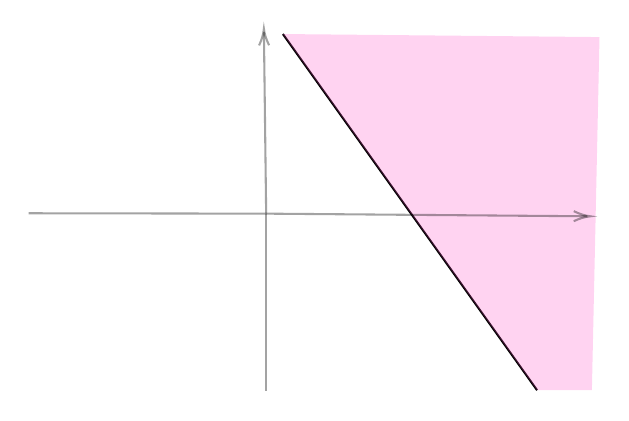
\begin{tikzpicture}[x=0.55pt,y=0.55pt,yscale=-1,xscale=1]
%uncomment if require: \path (0,300); %set diagram left start at 0, and has height of 300

%Straight Lines [id:da834373648885985] 
\draw    (335,25.5) -- (502,259.5) ;
%Shape: Polygon [id:ds19097348090692345] 
\draw  [draw opacity=0][fill=myhotpink  ,fill opacity=0.25 ] (543,27.5) -- (538,259.5) -- (502,259.5) -- (335,25.5) -- cycle ;
%Straight Lines [id:da488242538610719] 
\draw [color={rgb, 255:red, 0; green, 0; blue, 0 }  ,draw opacity=0.36 ]   (324,143.5) -- (322.52,24) ;
\draw [shift={(322.5,22)}, rotate = 449.29] [color={rgb, 255:red, 0; green, 0; blue, 0 }  ,draw opacity=0.36 ][line width=0.75]    (10.93,-3.29) .. controls (6.95,-1.4) and (3.31,-0.3) .. (0,0) .. controls (3.31,0.3) and (6.95,1.4) .. (10.93,3.29)   ;
%Straight Lines [id:da1979668435494064] 
\draw [color={rgb, 255:red, 0; green, 0; blue, 0 }  ,draw opacity=0.36 ]   (324,143.5) -- (324,260.25) ;
%Straight Lines [id:da5494641877725677] 
\draw [color={rgb, 255:red, 0; green, 0; blue, 0 }  ,draw opacity=0.36 ]   (168,143.25) -- (324,143.5) ;
%Straight Lines [id:da7425835818655306] 
\draw [color={rgb, 255:red, 0; green, 0; blue, 0 }  ,draw opacity=0.36 ]   (324,143.5) -- (535,145.23) ;
\draw [shift={(537,145.25)}, rotate = 180.47] [color={rgb, 255:red, 0; green, 0; blue, 0 }  ,draw opacity=0.36 ][line width=0.75]    (10.93,-3.29) .. controls (6.95,-1.4) and (3.31,-0.3) .. (0,0) .. controls (3.31,0.3) and (6.95,1.4) .. (10.93,3.29)   ;

\end{tikzpicture}

\end{center} 
% \caption{Visualization of trajectory generation done in the developed software}
\end{figure}

 
\end{flushleft}
\end{frame}



\begin{frame}{Half-spaces}
\framesubtitle{Construction. Simple case}
\begin{flushleft}

Consider half-space that passes through the origin, and defined by its normal vector $\mathbf{n}$:

\begin{figure} [h!]
\begin{center}

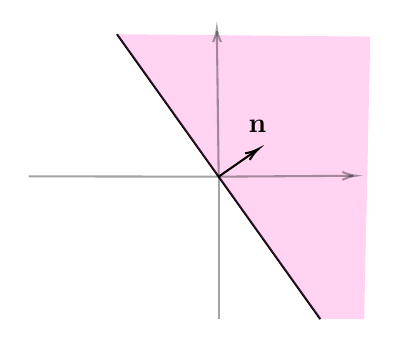
\begin{tikzpicture}[x=0.55pt,y=0.55pt,yscale=-0.8,xscale=0.8]
%uncomment if require: \path (0,300); %set diagram left start at 0, and has height of 300

%Straight Lines [id:da1372427179584501] 
\draw    (240.5,26.5) -- (407.5,260.5) ;
%Shape: Polygon [id:ds8874131334922846] 
\draw  [draw opacity=0][fill=myhotpink  ,fill opacity=0.25 ] (448.5,28.5) -- (443.5,260.5) -- (407.5,260.5) -- (240.5,26.5) -- cycle ;
%Straight Lines [id:da26449316913638876] 
\draw [color={rgb, 255:red, 0; green, 0; blue, 0 }  ,draw opacity=0.36 ]   (324,143.5) -- (322.52,24) ;
\draw [shift={(322.5,22)}, rotate = 449.29] [color={rgb, 255:red, 0; green, 0; blue, 0 }  ,draw opacity=0.36 ][line width=0.75]    (10.93,-3.29) .. controls (6.95,-1.4) and (3.31,-0.3) .. (0,0) .. controls (3.31,0.3) and (6.95,1.4) .. (10.93,3.29)   ;
%Straight Lines [id:da016556578057246085] 
\draw [color={rgb, 255:red, 0; green, 0; blue, 0 }  ,draw opacity=0.36 ]   (324,143.5) -- (324,260.25) ;
%Straight Lines [id:da9632237782300941] 
\draw [color={rgb, 255:red, 0; green, 0; blue, 0 }  ,draw opacity=0.36 ]   (168,143.25) -- (324,143.5) ;
%Straight Lines [id:da7562358617725318] 
\draw [color={rgb, 255:red, 0; green, 0; blue, 0 }  ,draw opacity=0.36 ]   (324,143.5) -- (434.5,142.76) ;
\draw [shift={(436.5,142.75)}, rotate = 539.62] [color={rgb, 255:red, 0; green, 0; blue, 0 }  ,draw opacity=0.36 ][line width=0.75]    (10.93,-3.29) .. controls (6.95,-1.4) and (3.31,-0.3) .. (0,0) .. controls (3.31,0.3) and (6.95,1.4) .. (10.93,3.29)   ;
%Straight Lines [id:da5203882996773224] 
\draw    (324,143.5) -- (354.96,121.94) ;
\draw [shift={(356.6,120.8)}, rotate = 505.15] [color={rgb, 255:red, 0; green, 0; blue, 0 }  ][line width=0.75]    (10.93,-3.29) .. controls (6.95,-1.4) and (3.31,-0.3) .. (0,0) .. controls (3.31,0.3) and (6.95,1.4) .. (10.93,3.29)   ;

% Text Node
\draw (346,94.6) node [anchor=north west][inner sep=0.75pt]    {$\mathbf{n}$};
\end{tikzpicture}

\end{center} 
% \caption{Visualization of trajectory generation done in the developed software}
\end{figure}


It is easy to see that this half-space can be defined as "all vectors $\mathbf{x}$, such that $\mathbf{n} \cdot \mathbf{x} \leq 0$", which is the same as using $\mathbf{n}$ instead of $\mathbf{a}$ in our original definition, setting $b = 0$.
 
\end{flushleft}
\end{frame}




\begin{frame}{Half-spaces}
\framesubtitle{Construction. General case}
\begin{flushleft}

In the general case there is some distance between the boundary of the half-space and the origin, let's say $d$.

\begin{figure} [h!]
\begin{center}

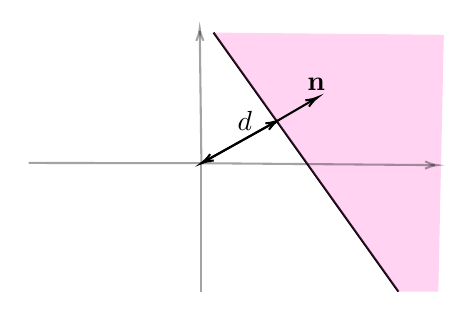
\begin{tikzpicture}[x=0.50pt,y=0.50pt,yscale=-0.8,xscale=0.8]
%uncomment if require: \path (0,300); %set diagram left start at 0, and has height of 300

%Straight Lines [id:da2789966724055237] 
\draw    (335,25.5) -- (502,259.5) ;
%Shape: Polygon [id:ds38542560237622214] 
\draw  [draw opacity=0][fill=myhotpink  ,fill opacity=0.25 ] (543,27.5) -- (538,259.5) -- (502,259.5) -- (335,25.5) -- cycle ;
%Straight Lines [id:da1318799276011975] 
\draw    (324,143.5) -- (391.25,105.97) ;
\draw [shift={(393,105)}, rotate = 510.84] [color={rgb, 255:red, 0; green, 0; blue, 0 }  ][line width=0.75]    (10.93,-3.29) .. controls (6.95,-1.4) and (3.31,-0.3) .. (0,0) .. controls (3.31,0.3) and (6.95,1.4) .. (10.93,3.29)   ;
%Straight Lines [id:da16726546442154655] 
\draw    (393,105) -- (427.27,85.01) ;
\draw [shift={(429,84)}, rotate = 509.74] [color={rgb, 255:red, 0; green, 0; blue, 0 }  ][line width=0.75]    (10.93,-3.29) .. controls (6.95,-1.4) and (3.31,-0.3) .. (0,0) .. controls (3.31,0.3) and (6.95,1.4) .. (10.93,3.29)   ;
%Straight Lines [id:da3700435560461126] 
\draw [color={rgb, 255:red, 0; green, 0; blue, 0 }  ,draw opacity=0.36 ]   (324,143.5) -- (322.52,24) ;
\draw [shift={(322.5,22)}, rotate = 449.29] [color={rgb, 255:red, 0; green, 0; blue, 0 }  ,draw opacity=0.36 ][line width=0.75]    (10.93,-3.29) .. controls (6.95,-1.4) and (3.31,-0.3) .. (0,0) .. controls (3.31,0.3) and (6.95,1.4) .. (10.93,3.29)   ;
%Straight Lines [id:da802723255513649] 
\draw [color={rgb, 255:red, 0; green, 0; blue, 0 }  ,draw opacity=0.36 ]   (324,143.5) -- (324,260.25) ;
%Straight Lines [id:da6699382328755694] 
\draw [color={rgb, 255:red, 0; green, 0; blue, 0 }  ,draw opacity=0.36 ]   (168,143.25) -- (324,143.5) ;
%Straight Lines [id:da17215887220844728] 
\draw [color={rgb, 255:red, 0; green, 0; blue, 0 }  ,draw opacity=0.36 ]   (324,143.5) -- (535,145.23) ;
\draw [shift={(537,145.25)}, rotate = 180.47] [color={rgb, 255:red, 0; green, 0; blue, 0 }  ,draw opacity=0.36 ][line width=0.75]    (10.93,-3.29) .. controls (6.95,-1.4) and (3.31,-0.3) .. (0,0) .. controls (3.31,0.3) and (6.95,1.4) .. (10.93,3.29)   ;
%Straight Lines [id:da7790488401292512] 
\draw    (393,105) -- (325.75,142.53) ;
\draw [shift={(324,143.5)}, rotate = 330.84000000000003] [color={rgb, 255:red, 0; green, 0; blue, 0 }  ][line width=0.75]    (10.93,-3.29) .. controls (6.95,-1.4) and (3.31,-0.3) .. (0,0) .. controls (3.31,0.3) and (6.95,1.4) .. (10.93,3.29)   ;

% Text Node
\draw (417,64) node [anchor=north west][inner sep=0.75pt]    {$\mathbf{n}$};
% Text Node
\draw (354,94) node [anchor=north west][inner sep=0.75pt]    {$d$};

\end{tikzpicture}

\end{center} 
% \caption{Visualization of trajectory generation done in the developed software}
\end{figure}

%
Here the half space can be defined as "all vectors $\mathbf{x}$, such that $\mathbf{x}^\top \frac{\mathbf{n}}{|| \mathbf{n} ||}  \leq d$". This is the same as making $\mathbf{a} = \mathbf{n}$ and $b = d ||\mathbf{a}||$.
 
\end{flushleft}
\end{frame}



\begin{frame}{Half-spaces}
\framesubtitle{Combination}
\begin{flushleft}

We can define a region of space as an \emph{intersection} of half-spaces $\mathbf{a}_i^\top \mathbf{x} \leq b_i$:

\begin{figure} [h!]
\begin{center}
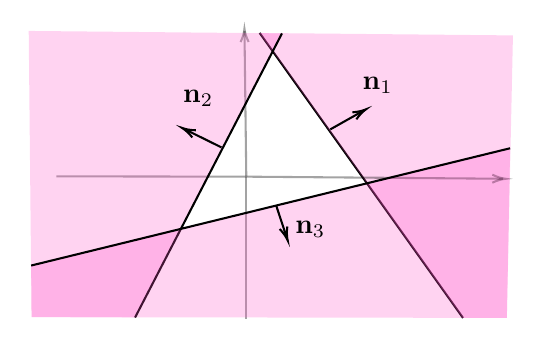
\begin{tikzpicture}[x=0.55pt,y=0.55pt,yscale=-0.8,xscale=0.8]
%uncomment if require: \path (0,300); %set diagram left start at 0, and has height of 300

%Straight Lines [id:da6725207022045878] 
\draw    (335,25.5) -- (502,259.5) ;
%Shape: Polygon [id:ds5954714579613014] 
\draw  [draw opacity=0][fill=myhotpink  ,fill opacity=0.25 ] (543,27.5) -- (538,259.5) -- (502,259.5) -- (335,25.5) -- cycle ;
%Straight Lines [id:da6659527637106164] 
\draw    (393,104.67) -- (420.59,89.15) ;
\draw [shift={(422.33,88.17)}, rotate = 510.64] [color={rgb, 255:red, 0; green, 0; blue, 0 }  ][line width=0.75]    (10.93,-3.29) .. controls (6.95,-1.4) and (3.31,-0.3) .. (0,0) .. controls (3.31,0.3) and (6.95,1.4) .. (10.93,3.29)   ;
%Straight Lines [id:da7520623163425082] 
\draw [color={rgb, 255:red, 0; green, 0; blue, 0 }  ,draw opacity=0.36 ]   (324,143.5) -- (322.52,24) ;
\draw [shift={(322.5,22)}, rotate = 449.29] [color={rgb, 255:red, 0; green, 0; blue, 0 }  ,draw opacity=0.36 ][line width=0.75]    (10.93,-3.29) .. controls (6.95,-1.4) and (3.31,-0.3) .. (0,0) .. controls (3.31,0.3) and (6.95,1.4) .. (10.93,3.29)   ;
%Straight Lines [id:da8019604271716267] 
\draw [color={rgb, 255:red, 0; green, 0; blue, 0 }  ,draw opacity=0.36 ]   (324,143.5) -- (324,260.25) ;
%Straight Lines [id:da9975734887022978] 
\draw [color={rgb, 255:red, 0; green, 0; blue, 0 }  ,draw opacity=0.36 ]   (168,143.25) -- (324,143.5) ;
%Straight Lines [id:da6037170480132432] 
\draw [color={rgb, 255:red, 0; green, 0; blue, 0 }  ,draw opacity=0.36 ]   (324,143.5) -- (535,145.23) ;
\draw [shift={(537,145.25)}, rotate = 180.47] [color={rgb, 255:red, 0; green, 0; blue, 0 }  ,draw opacity=0.36 ][line width=0.75]    (10.93,-3.29) .. controls (6.95,-1.4) and (3.31,-0.3) .. (0,0) .. controls (3.31,0.3) and (6.95,1.4) .. (10.93,3.29)   ;
%Shape: Polygon [id:ds2697615572268972] 
\draw  [draw opacity=0][fill=myhotpink  ,fill opacity=0.25 ] (353.33,25.83) -- (232.67,259.17) -- (147.67,258.83) -- (145.33,23.83) -- cycle ;
%Straight Lines [id:da5531097421453206] 
\draw    (353.33,25.83) -- (232.67,259.17) ;
%Shape: Polygon [id:ds45225811581456] 
\draw  [draw opacity=0][fill=myhotpink  ,fill opacity=0.25 ] (540.67,120.17) -- (538,259.5) -- (147.67,258.83) -- (147.33,216.5) -- cycle ;
%Straight Lines [id:da2591402586511129] 
\draw    (540.67,120.17) -- (147.33,216.5) ;
%Straight Lines [id:da6357606107432212] 
\draw    (303.67,119.5) -- (273.13,104.39) ;
\draw [shift={(271.33,103.5)}, rotate = 386.33000000000004] [color={rgb, 255:red, 0; green, 0; blue, 0 }  ][line width=0.75]    (10.93,-3.29) .. controls (6.95,-1.4) and (3.31,-0.3) .. (0,0) .. controls (3.31,0.3) and (6.95,1.4) .. (10.93,3.29)   ;
%Straight Lines [id:da663892331852407] 
\draw    (348.67,167.5) -- (357.37,193.93) ;
\draw [shift={(358,195.83)}, rotate = 251.76999999999998] [color={rgb, 255:red, 0; green, 0; blue, 0 }  ][line width=0.75]    (10.93,-3.29) .. controls (6.95,-1.4) and (3.31,-0.3) .. (0,0) .. controls (3.31,0.3) and (6.95,1.4) .. (10.93,3.29)   ;

% Text Node
\draw (417,59) node [anchor=north west][inner sep=0.75pt]    {$\mathbf n_{1}$};
% Text Node
\draw (269.67,70) node [anchor=north west][inner sep=0.75pt]    {$\mathbf n_{2}$};
% Text Node
\draw (361.67,177.67) node [anchor=north west][inner sep=0.75pt]    {$\mathbf n_{3}$};

\end{tikzpicture}

\end{center} 
% \caption{Visualization of trajectory generation done in the developed software}
\end{figure}


Resulting region will be easily described as $\begin{bmatrix} \mathbf{a}_1^\top \\ ... \\ \mathbf{a}_k^\top \end{bmatrix} \mathbf{x} \leq \begin{bmatrix} b_1 \\ ... \\ b_k \end{bmatrix}$

 
\end{flushleft}
\end{frame}


\begin{frame}{Half-spaces}
\framesubtitle{H-representation}
\begin{flushleft}

The last result allows us to write any convex polytope as a matrix inequality:

\begin{equation}
\label{eq:ineq} 
    \mathbf{A} \mathbf{x} \leq  \mathbf{b} 
\end{equation}

And conversely, any matrix inequality \eqref{eq:ineq} represents either an empty set or a convex polytope.

\bigskip

\begin{definition}
 $\mathbf{A} \mathbf{x} \leq  \mathbf{b}$ is called \emph{H-representation} of a polytope.
\end{definition}
 
\end{flushleft}
\end{frame}



\begin{frame}{V-representation}
% \framesubtitle{}
\begin{flushleft}

Convex polytopes have alternative representations, such as \emph{V-representation}. In amounts to representing polytope as a set of its vertices.

\begin{example}
$V = \begin{bmatrix} -1 & -1 & 1 & 1 \\ -1 & 1 & 1 & -1 \end{bmatrix}$ is a V-representation of a square.
\end{example}

\begin{example}
$\begin{bmatrix} 1 & 0 \\ 0 & 1 \\ -1 & 0 \\ 0 & -1 \end{bmatrix}
\begin{bmatrix} x_1 \\ x_2 \end{bmatrix} \leq
\begin{bmatrix} 1 \\ 1 \\ 1 \\ 1 \end{bmatrix}$
is an H-representation of the same square.
\end{example}
 
\end{flushleft}
\end{frame}



\begin{frame}{H and V-representations}
% \framesubtitle{}
\begin{flushleft}

Question: can we use V-representation for non-convex polytopes? What about H-representation?

\bigskip

Another note: to transfer from H-representation to V-representation, you need to solve \emph{vertex enumeration} problem, which is computationally expensive.
 
\end{flushleft}
\end{frame}




\begin{frame}{Linear approximation of convex regions}
% \framesubtitle{Parameter estimation}
\begin{flushleft}
Some convex regions can be easily approximated using polytopes.

\begin{figure} [h!]
\begin{center}

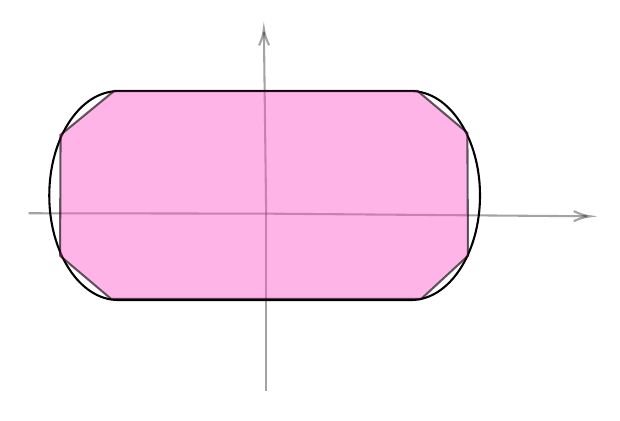
\begin{tikzpicture}[x=0.55pt,y=0.55pt,yscale=-1,xscale=1]
%uncomment if require: \path (0,300); %set diagram left start at 0, and has height of 300

%Straight Lines [id:da10201365463278256] 
\draw [color={rgb, 255:red, 0; green, 0; blue, 0 }  ,draw opacity=0.36 ]   (324,143.5) -- (322.52,24) ;
\draw [shift={(322.5,22)}, rotate = 449.29] [color={rgb, 255:red, 0; green, 0; blue, 0 }  ,draw opacity=0.36 ][line width=0.75]    (10.93,-3.29) .. controls (6.95,-1.4) and (3.31,-0.3) .. (0,0) .. controls (3.31,0.3) and (6.95,1.4) .. (10.93,3.29)   ;
%Straight Lines [id:da6957790210068775] 
\draw [color={rgb, 255:red, 0; green, 0; blue, 0 }  ,draw opacity=0.36 ]   (324,143.5) -- (324,260.25) ;
%Straight Lines [id:da17513960825207286] 
\draw [color={rgb, 255:red, 0; green, 0; blue, 0 }  ,draw opacity=0.36 ]   (168,143.25) -- (324,143.5) ;
%Straight Lines [id:da5820199298694646] 
\draw [color={rgb, 255:red, 0; green, 0; blue, 0 }  ,draw opacity=0.36 ]   (324,143.5) -- (535,145.23) ;
\draw [shift={(537,145.25)}, rotate = 180.47] [color={rgb, 255:red, 0; green, 0; blue, 0 }  ,draw opacity=0.36 ][line width=0.75]    (10.93,-3.29) .. controls (6.95,-1.4) and (3.31,-0.3) .. (0,0) .. controls (3.31,0.3) and (6.95,1.4) .. (10.93,3.29)   ;
%Flowchart: Terminator [id:dp7571888204896569] 
\draw   (226.78,63) -- (419.22,63) .. controls (444.23,63) and (464.5,93.72) .. (464.5,131.63) .. controls (464.5,169.53) and (444.23,200.25) .. (419.22,200.25) -- (226.78,200.25) .. controls (201.77,200.25) and (181.5,169.53) .. (181.5,131.63) .. controls (181.5,93.72) and (201.77,63) .. (226.78,63) -- cycle ;
%Shape: Polygon [id:ds9338072370258934] 
\draw  [color={rgb, 255:red, 0; green, 0; blue, 0 }  ,draw opacity=0.62 ][fill=myhotpink  ,fill opacity=0.43 ] (224.2,62.8) -- (423.4,62.8) -- (456.2,90.4) -- (456.6,171.2) -- (425.8,199.6) -- (222.2,199.6) -- (188.6,171.2) -- (188.9,91.75) -- cycle ;
\end{tikzpicture}

\end{center} 
% \caption{Visualization of trajectory generation done in the developed software}
\end{figure}


Which allows to represent constraints on $\mathbf{x}$ to belong in such a region as a matrix inequality
 
\end{flushleft}
\end{frame}



\begin{frame}{Homework}
% \framesubtitle{Parameter estimation}
\begin{flushleft}

Represent in matrix inequality form the following figures:

\begin{itemize}
    \item Equilateral triangle
    \item A square
    \item Parallelepiped
    \item Trapezoid
\end{itemize}

\end{flushleft}
\end{frame}


% \begin{frame}{Self-study}
% % \framesubtitle{Part 3}
% \begin{flushleft}

% \begin{itemize}
%     \item \href{https://www.youtube.com/watch?v=kcOodzDGV4c}{Convex Optimization, lecture 3, S. Boyd. Stanford. Convex functions}.
% \end{itemize}

% \end{flushleft}
% \end{frame}



\begin{frame}
	\centerline{Lecture slides are available via Moodle.}
	\bigskip
	\centerline{You can help improve these slides at:}
	\centerline{
		\mygit
	}
	\bigskip
	
	\textcolor{black}{\qrcode[height=1.5in]{https://github.com/SergeiSa/Computational-Intelligence-Slides-Spring-2022}}
	\bigskip
	
	
	\centerline{Check Moodle for additional links, videos, textbook suggestions.}
\end{frame}

\end{document}
